\documentclass[12pt]{article}
\usepackage{graphicx} % Required for inserting images
\usepackage[utf8]{lipsum, inputenc}
\usepackage[margin=1in]{geometry}
\usepackage{adjustbox} % for adjusting table dimensions
\usepackage{booktabs} % Used to create tables
\usepackage{tabu} % Also used to create tables
\usepackage{fancyhdr}
\usepackage{hyperref}
% \usepackage{subcaption}
\usepackage[style=chem-acs, articletitle=true]{biblatex}
\addbibresource{references.bib}
\usepackage{subfigure}

\title{Student Test Score Prediction w/ Linear Regression}
\author{Giorgos Tzimas }
\date{June 2023}

\begin{document}

\maketitle


\section{Dataset Description}
\subsection{Background}
The panel dataset contains cross-section data from the High School and Beyond survey conducted by the Department of Education in 1980. The data was collected in order to study the relationship between early high school experiences and the students' educational experiences in high school and after, as well as the effects of how family, community, school and classroom factors affect student performance.\\ \\
For further information: \textbf{https://nces.ed.gov/surveys/hsb/}

\subsection{Observations and Attributes}
The dataset comprises of \textbf{4,739} entries with \textbf{15} distinct features. These features contain a range of information pertaining to both the student, the school they attend and their parents.

\begin{table}[h]
    \centering
    \begin{tabu}{ll}
\toprule
 & Description \\
Feature &  \\
\midrule
gender & Student's gender \\
ethnicity & Student's ethnicity (African-American, Hispanic or other) \\
score & Base year composite test score \\
fcollege & Is the father a college graduate? \\
mcollege & Is the mother a college graduate? \\
home & Does the family own their home? \\
urban & Is the school in an urban area? \\
unemp & County unemployment rate in 1980. \\
wage & State hourly wage in manufacturing in 1980. \\
distance & Distance from 4-year college (in 10 miles). \\
tuition & Average state 4-year college tuition (in 1000 USD). \\
education & Number of years of education. \\
income & Is the family income above USD 25,000 per year? \\
region & School region (West or other). \\
\bottomrule
\end{tabu}

    \caption{Dataset features and their descriptions}
    \label{tab:var_descriptions}
\end{table}

\vfill
\subsection{Data Types}
Out of the 15 features in the dataset:
\begin{itemize}
  \item 8 are of type "object" or text
  \item 2 are of type "integer"
  \item 5 are of type "float"
\end{itemize}

\begin{table}[h!]
    \centering
    \begin{tabu}{ll}
\toprule
 & Data Type \\
Feature &  \\
\midrule
ID & int64 \\
gender & object \\
ethnicity & object \\
score & float64 \\
fcollege & object \\
mcollege & object \\
home & object \\
urban & object \\
\bottomrule
\end{tabu}
    \begin{tabu}{ll}
\toprule
 & Data Type \\
Feature &  \\
\midrule
unemp & float64 \\
wage & float64 \\
distance & float64 \\
tuition & float64 \\
education & int64 \\
income & object \\
region & object \\
\bottomrule
\end{tabu}
    \caption{Dataset attributes and their types}
    \label{tab:dtypes}
\end{table}

\section{Data Cleaning}
None of our records or features in the dataset contain any missing values. Therefore, we will not have to use any imputation methods in this case.
\begin{table}[h]
    \centering
    \begin{tabu}{lr}
\toprule
 & # Missing \\
Feature &  \\
\midrule
ID & 0 \\
gender & 0 \\
ethnicity & 0 \\
score & 0 \\
fcollege & 0 \\
mcollege & 0 \\
home & 0 \\
urban & 0 \\
\bottomrule
\end{tabu}
    \begin{tabu}{lr}
\toprule
 & # Missing \\
Feature &  \\
\midrule
unemp & 0 \\
wage & 0 \\
distance & 0 \\
tuition & 0 \\
education & 0 \\
income & 0 \\
region & 0 \\
\bottomrule
\end{tabu}
    \caption{Features with number of missing values}
    \label{tab:missing}
\end{table}

\newpage
\section{Data Transformation}
All of the categorical variables in the dataset will be one-hot encoded (dummy-coded) into numeric variables with n-1 columns (n=number of levels in the feature).
\begin{itemize}
    \item n\_gender: 1 if "male", 0 if "female
    \item n\_ethnicity\_hispanic: 1 if "hispanic", 0 if otherwise
    \item n\_ethnicity\_afam: 1 if "afam", 0 if otherwise
    \item n\_fcollege: 1 if "yes", 0 if "no"
    \item n\_mcollege: 1 if "yes", 0 if "no"
    \item n\_home: 1 if "yes", 0 if "no"
    \item n\_urban: 1 if "yes", 0 if "no"
    \item n\_region: 1 if "west", 0 if "other"
\end{itemize}

\begin{table}[h]
    \centering
    \resizebox{1.1\textwidth}{!}{%
    \begin{tabu}{lrrrrrrrrrrrrrrrr}
\toprule
 & ID & score & unemp & wage & distance & tuition & education & n\_gender & n\_ethnicity\_afam & n\_ethnicity\_hispanic & n\_fcollege & n\_mcollege & home\_yes & urban\_yes & n\_income & n\_region \\
\midrule
0 & 1 & 39.150002 & 6.200000 & 8.090000 & 0.200000 & 0.889150 & 12 & 1 & 0 & 0 & 1 & 0 & 1 & 1 & 1 & 0 \\
1 & 2 & 48.869999 & 6.200000 & 8.090000 & 0.200000 & 0.889150 & 12 & 0 & 0 & 0 & 0 & 0 & 1 & 1 & 0 & 0 \\
2 & 3 & 48.740002 & 6.200000 & 8.090000 & 0.200000 & 0.889150 & 12 & 1 & 0 & 0 & 0 & 0 & 1 & 1 & 0 & 0 \\
3 & 4 & 40.400002 & 6.200000 & 8.090000 & 0.200000 & 0.889150 & 12 & 1 & 1 & 0 & 0 & 0 & 1 & 1 & 0 & 0 \\
4 & 5 & 40.480000 & 5.600000 & 8.090000 & 0.400000 & 0.889150 & 13 & 0 & 0 & 0 & 0 & 0 & 0 & 1 & 0 & 0 \\
\bottomrule
\end{tabu} }
    \caption{Dataset after dummy-coding}
    \label{tab:transformed_data}
\end{table}

\section{Exploratory Data Analysis}
In this section, we will visually explore our dataset to gain some insight into the relationships between different features.
\subsection{Correlation Matrix}
\begin{table}[h]
    \centering
    \renewcommand{\arraystretch}{1.5} % Increase the stretch factor to increase the vertical spacing
    \resizebox{1.1\textwidth}{!}{%
    \begin{tabu}{lrrrrrrrrrrrrrrr}
\toprule
 & score & unemp & wage & distance & tuition & education & n\_gender & n\_ethnicity\_afam & n\_ethnicity\_hispanic & n\_fcollege & n\_mcollege & home\_yes & urban\_yes & n\_income & n\_region \\
\midrule
score & 1.000000 & -0.025309 & 0.116627 & -0.067979 & 0.129858 & 0.465187 & 0.080169 & -0.284252 & -0.161187 & 0.250970 & 0.189563 & 0.125874 & -0.085139 & 0.178368 & -0.026034 \\
unemp & -0.025309 & 1.000000 & 0.266771 & 0.293036 & 0.184027 & -0.014746 & -0.028380 & -0.059376 & 0.088610 & -0.100055 & -0.086024 & 0.005036 & -0.052140 & -0.078126 & -0.041865 \\
wage & 0.116627 & 0.266771 & 1.000000 & -0.000390 & 0.317727 & 0.023858 & 0.027211 & -0.133696 & -0.099519 & 0.030929 & 0.016939 & 0.067455 & -0.032566 & 0.071773 & -0.083654 \\
distance & -0.067979 & 0.293036 & -0.000390 & 1.000000 & -0.100981 & -0.093183 & -0.003441 & -0.100022 & 0.058226 & -0.105474 & -0.081523 & 0.019605 & -0.289175 & -0.080422 & 0.068089 \\
tuition & 0.129858 & 0.184027 & 0.317727 & -0.100981 & 1.000000 & 0.039534 & 0.009025 & 0.059007 & -0.304375 & 0.028796 & 0.036125 & -0.000320 & -0.016181 & 0.053930 & -0.582348 \\
education & 0.465187 & -0.014746 & 0.023858 & -0.093183 & 0.039534 & 1.000000 & 0.009764 & -0.090034 & -0.043374 & 0.284356 & 0.225177 & 0.096519 & -0.015005 & 0.219166 & -0.024145 \\
n\_gender & 0.080169 & -0.028380 & 0.027211 & -0.003441 & 0.009025 & 0.009764 & 1.000000 & -0.039639 & 0.018810 & 0.040697 & 0.019911 & 0.038162 & 0.009728 & 0.058891 & -0.013418 \\
n\_ethnicity\_afam & -0.284252 & -0.059376 & -0.133696 & -0.100022 & 0.059007 & -0.090034 & -0.039639 & 1.000000 & -0.216348 & -0.101376 & -0.018085 & -0.126593 & 0.183720 & -0.096960 & -0.144095 \\
n\_ethnicity\_hispanic & -0.161187 & 0.088610 & -0.099519 & 0.058226 & -0.304375 & -0.043374 & 0.018810 & -0.216348 & 1.000000 & -0.112351 & -0.106208 & -0.063879 & 0.077073 & -0.128255 & 0.207679 \\
n\_fcollege & 0.250970 & -0.100055 & 0.030929 & -0.105474 & 0.028796 & 0.284356 & 0.040697 & -0.101376 & -0.112351 & 1.000000 & 0.429710 & 0.077525 & -0.052510 & 0.353563 & 0.029686 \\
n\_mcollege & 0.189563 & -0.086024 & 0.016939 & -0.081523 & 0.036125 & 0.225177 & 0.019911 & -0.018085 & -0.106208 & 0.429710 & 1.000000 & 0.063916 & -0.034306 & 0.245670 & -0.011578 \\
home\_yes & 0.125874 & 0.005036 & 0.067455 & 0.019605 & -0.000320 & 0.096519 & 0.038162 & -0.126593 & -0.063879 & 0.077525 & 0.063916 & 1.000000 & -0.096868 & 0.138826 & 0.004868 \\
urban\_yes & -0.085139 & -0.052140 & -0.032566 & -0.289175 & -0.016181 & -0.015005 & 0.009728 & 0.183720 & 0.077073 & -0.052510 & -0.034306 & -0.096868 & 1.000000 & -0.071642 & -0.052117 \\
n\_income & 0.178368 & -0.078126 & 0.071773 & -0.080422 & 0.053930 & 0.219166 & 0.058891 & -0.096960 & -0.128255 & 0.353563 & 0.245670 & 0.138826 & -0.071642 & 1.000000 & 0.007449 \\
n\_region & -0.026034 & -0.041865 & -0.083654 & 0.068089 & -0.582348 & -0.024145 & -0.013418 & -0.144095 & 0.207679 & 0.029686 & -0.011578 & 0.004868 & -0.052117 & 0.007449 & 1.000000 \\
\bottomrule
\end{tabu} }
    \caption{Correlation matrix for all features}
    \label{tab:corr_matrix}
\end{table}
\newpage
\begin{itemize}
    \item None of our independent variables are strongly correlated with each other, which suggests multicollinearity might not be an issue when building the model
    \item The feature with the strongest correlation to our dependent variable (score) is education (0.46)
    \item The second strongest correlated variable with score is n\_ethnicity\_afam (-0.28)
\end{itemize}

\subsection{Distribution of "score"}

\begin{figure}[h]
    \centering
    \begin{minipage}[t]{0.65\textwidth}
        \vspace{0pt}
        \centering
        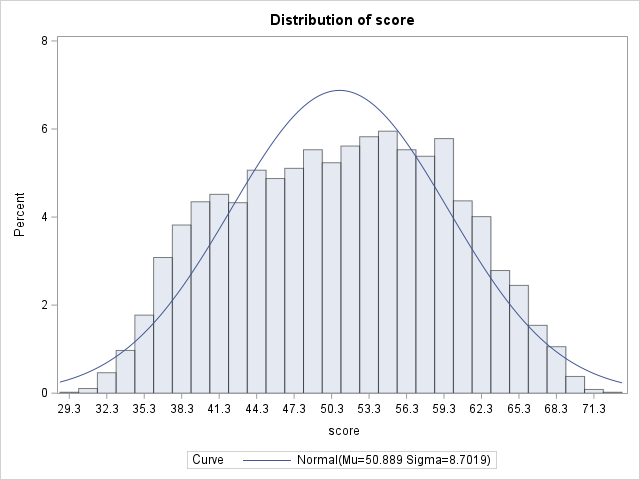
\includegraphics[width=\textwidth]{images/score_hist.png}
        \caption{Distribution of variable "score"}
        \label{fig:score_dist}
    \end{minipage}\hfill
    \begin{minipage}[t]{0.3\textwidth}
        \vspace{15pt}
        \centering
        \begin{tabu}{lr}
\toprule
 & Values \\
Measure &  \\
\midrule
Mean & 50.889029 \\
Median & 51.189999 \\
Mode & 56.020000 \\
St. Dev. & 8.700991 \\
Variance & 75.707252 \\
Min & 28.950001 \\
Max & 72.809998 \\
Range & 43.859997 \\
IQR & 13.844999 \\
Skew & -0.032655 \\
\bottomrule
\end{tabu}
        \caption{Location and variability metrics}
        \label{fig:score_measures}
    \end{minipage}
    \label{fig:score_fig}
\end{figure}

\begin{itemize}
    \item Our dependent variable is normally distributed with a negligible skewness of -0.03
    \item The mean score for all students is 50.89
    \item The standard deviation for student score is 8.7
    \item The lowest score is 28.95 and the largest is 72.81
\end{itemize}

\subsection{Distribution of "unemp"}
\begin{figure}[h]
    \centering
    \begin{minipage}[t]{0.65\textwidth}
        \vspace{0pt}
        \centering
        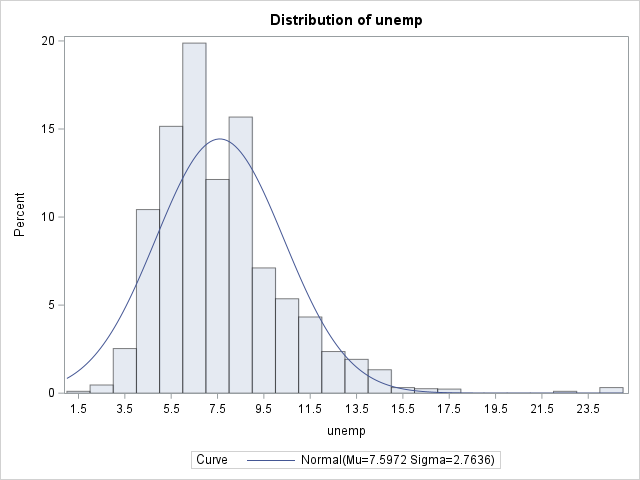
\includegraphics[width=\textwidth]{images/unemp_hist.png}
        \caption{Distribution of variable "unemp"}
        \label{fig:unemp_dist}
    \end{minipage}\hfill
    \begin{minipage}[t]{0.3\textwidth}
        \vspace{15pt}
        \centering
        \begin{tabu}{lr}
\toprule
 & Values \\
Measure &  \\
\midrule
Mean & 7.597215 \\
Median & 7.100000 \\
Mode & 8.000000 \\
St. Dev. & 2.763289 \\
Variance & 7.635768 \\
Min & 1.400000 \\
Max & 24.900000 \\
Range & 23.500000 \\
IQR & 3.000000 \\
Skew & 1.558486 \\
\bottomrule
\end{tabu}
        \caption{Location and variability metrics}
        \label{fig:unemp_measures}
    \end{minipage}
    \label{fig:unemp_fig}
\end{figure}

\begin{itemize}
    \item The county unemployment rate is right-tailed with a skewness of 1.56
    \item The mean unemployment rate is 7.60 and the median is 7.1
    \item The standard deviation is 2.76
    \item The lowest unemployment rate is 1.40 and the largest is 24.90
    \item This distribution's right-skewness is due to potentially outlier values in the [21.5, 24.9] range
    \item We will take the log of "unemp" and compare its distribution to the original
\end{itemize}
\newpage
\begin{figure}[h]
    \centering
    \begin{minipage}[t]{0.65\textwidth}
        \vspace{0pt}
        \centering
        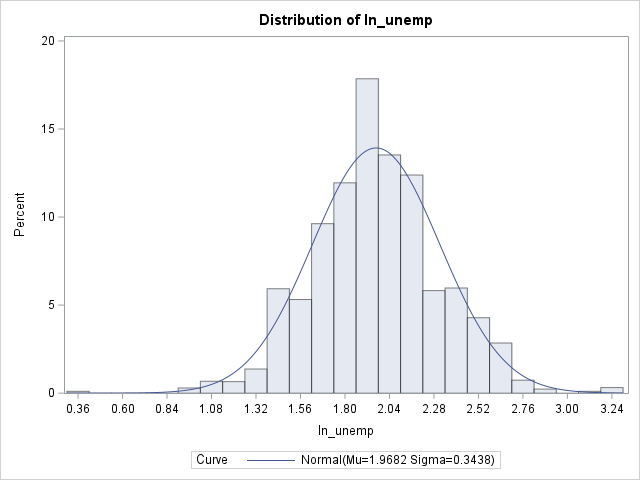
\includegraphics[width=\textwidth]{images/ln_unemp_hist.png}
        \caption{Distribution of variable "ln\_unemp"}
        \label{fig:ln_unemp_dist}
    \end{minipage}\hfill
    \begin{minipage}[t]{0.3\textwidth}
        \vspace{15pt}
        \centering
        \begin{tabu}{lr}
\toprule
 & Values \\
Measure &  \\
\midrule
Mean & 1.968177 \\
Median & 1.960095 \\
Mode & 2.079442 \\
St. Dev. & 0.343759 \\
Variance & 0.118170 \\
Min & 0.336472 \\
Max & 3.214868 \\
Range & 2.878396 \\
IQR & 0.411099 \\
Skew & 0.017166 \\
\bottomrule
\end{tabu}
        \caption{Location and variability metrics}
        \label{fig:ln_unemp_measures}
    \end{minipage}
    \label{fig:ln_unemp_fig}
\end{figure}
\begin{itemize}
    \item The right-tailedness of the original variable is mitigated by taking its natural logarithm with a new skew of 0.02
\end{itemize}

\subsection{Distribution of "wage"}
\begin{figure}[h]
    \centering
    \begin{minipage}[t]{0.65\textwidth}
        \vspace{0pt}
        \centering
        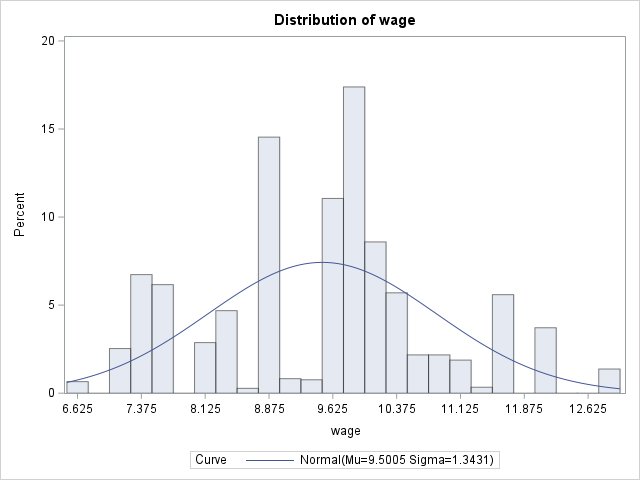
\includegraphics[width=\textwidth]{images/wage_hist.png}
        \caption{Distribution of variable "wage"}
        \label{fig:wage_dist}
    \end{minipage}\hfill
    \begin{minipage}[t]{0.3\textwidth}
        \vspace{15pt}
        \centering
        \begin{tabu}{lr}
\toprule
 & Values \\
Measure &  \\
\midrule
Mean & 9.500506 \\
Median & 9.680000 \\
Mode & 8.890000 \\
St. Dev. & 1.342925 \\
Variance & 1.803449 \\
Min & 6.590000 \\
Max & 12.960000 \\
Range & 6.370000 \\
IQR & 1.299999 \\
Skew & 0.093066 \\
\bottomrule
\end{tabu}
        \caption{Location and variability metrics}
        \label{fig:wage_measures}
    \end{minipage}
    \label{fig:wage_fig}
\end{figure}
\newpage
\begin{itemize}
    \item The hourly manufacturing wage is approximately normally distributed with a skewness of 0.09
    \item The mean wage is 9.50 and the median is 9.68
    \item The standard deviation is 
    \item The tails of the distribution are "fatter" than a standard normal distribution
    \item The lowest wage is 6.59 and the largest is 12.96
\end{itemize}

\subsection{Distribution of "distance"}
\begin{figure}[h]
    \centering
    \begin{minipage}[t]{0.65\textwidth}
        \vspace{0pt}
        \centering
        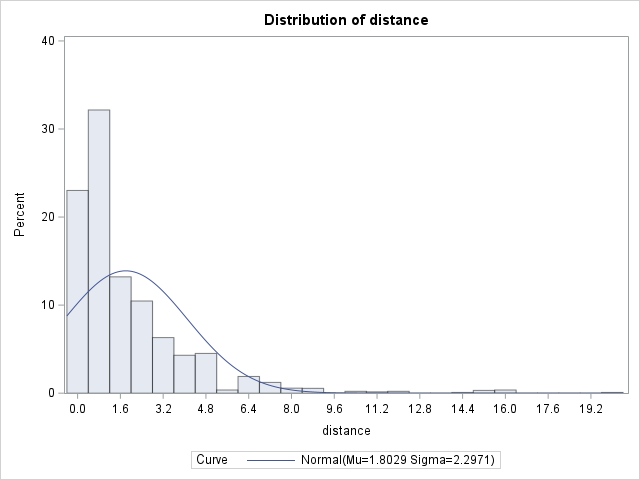
\includegraphics[width=\textwidth]{images/distance_hist.png}
        \caption{Distribution of variable "distance"}
        \label{fig:distance_dist}
    \end{minipage}\hfill
    \begin{minipage}[t]{0.3\textwidth}
        \vspace{15pt}
        \centering
        \begin{tabu}{lr}
\toprule
 & Values \\
Measure &  \\
\midrule
Mean & 1.802870 \\
Median & 1.000000 \\
Mode & 0.500000 \\
St. Dev. & 2.296885 \\
Variance & 5.275683 \\
Min & 0.000000 \\
Max & 20.000000 \\
Range & 20.000000 \\
IQR & 2.100000 \\
Skew & 2.999513 \\
\bottomrule
\end{tabu}
        \caption{Location and variability metrics}
        \label{fig:distance_measures}
    \end{minipage}
    \label{fig:distance_fig}
\end{figure}
\newpage
\begin{itemize}
    \item Distance from college in 10 miles is heavily right-tailed with a skewness of 3.00
    \item The mean distance is 1.8 (18 miles) and the median is 1.0 (10 miles)
    \item The standard deviation is 2.3 (23 miles)
    \item The lowest distance is 0.26 (2.6 miles) and the highest is 1.40 (14 miles)
    \item This distribution's right-skewness is due to potentially outlier values in the [8.5, 20] range
    \item Same as with "unemp", we will take the natural log of this feature
\end{itemize}

\begin{figure}[h]
    \centering
    \begin{minipage}[t]{0.65\textwidth}
        \vspace{0pt}
        \centering
        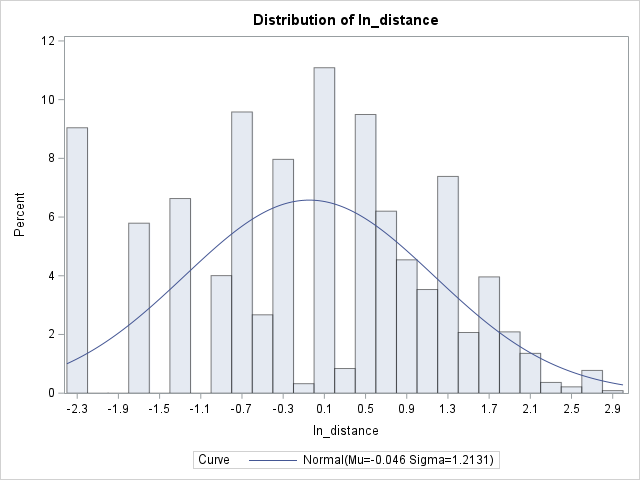
\includegraphics[width=\textwidth]{images/ln_distance_hist.png}
        \caption{Distribution of variable "distance"}
        \label{fig:ln_distance_dist}
    \end{minipage}\hfill
    \begin{minipage}[t]{0.3\textwidth}
        \vspace{15pt}
        \centering
        \begin{tabu}{lr}
\toprule
 & Values \\
Measure &  \\
\midrule
Mean & -0.045369 \\
Median & 0.000000 \\
Mode & 0.000000 \\
St. Dev. & 1.200915 \\
Variance & 1.442198 \\
Min & -2.302585 \\
Max & 2.995732 \\
Range & 5.298317 \\
IQR & 1.609438 \\
Skew & -0.143513 \\
\bottomrule
\end{tabu}

        \caption{Location and variability metrics}
        \label{fig:ln_distance_measures}
    \end{minipage}
    \label{fig:ln_distance_fig}
\end{figure}
\newpage
\begin{itemize}
    \item The right-tailedness of the original variable is mitigated by taking its natural logarithm with a new skew of -0.14
\end{itemize}

\subsection{Distribution of "tuition"}
\begin{figure}[h]
    \centering
    \begin{minipage}[t]{0.65\textwidth}
        \vspace{0pt}
        \centering
        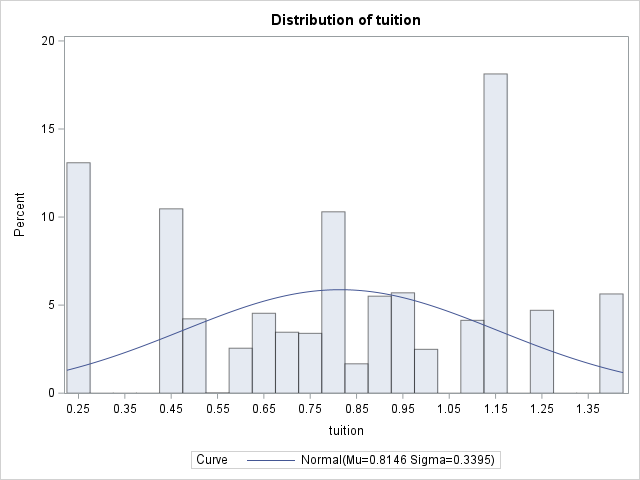
\includegraphics[width=\textwidth]{images/tuition_hist.png}
        \caption{Distribution of variable "distance"}
        \label{fig:tuition_dist}
    \end{minipage}\hfill
    \begin{minipage}[t]{0.3\textwidth}
        \vspace{15pt}
        \centering
        \begin{tabu}{lr}
\toprule
 & Values \\
Measure &  \\
\midrule
Mean & 0.814608 \\
Median & 0.824480 \\
Mode & 0.257510 \\
St. Dev. & 0.339468 \\
Variance & 0.115239 \\
Min & 0.257510 \\
Max & 1.404160 \\
Range & 1.146650 \\
IQR & 0.642030 \\
Skew & -0.151913 \\
\bottomrule
\end{tabu}
        \caption{Location and variability metrics}
        \label{fig:tuition_measures}
    \end{minipage}
    \label{fig:tuition_fig}
\end{figure}
\newpage

\begin{itemize}
    \item Four year college tuition in \$1000 is approximately normally distributed with a skewness of -0.15
    \item The mean tuition amount is 0.81 (\$810) and the median is 0.82 (\$820)
    \item The standard deviation is 0.34 (\$340)
    \item The lowest tuition amount is 0.26 (\$260) and the largest is 1.40 (\$1,400)
    \item The tails of the distribution are "fatter" than a standard normal distribution, suggesting many records present towards the tails and potential outliers
\end{itemize}
\newpage
\subsection{Distribution of "score" by Gender}
\begin{figure}[h]
    \centering
    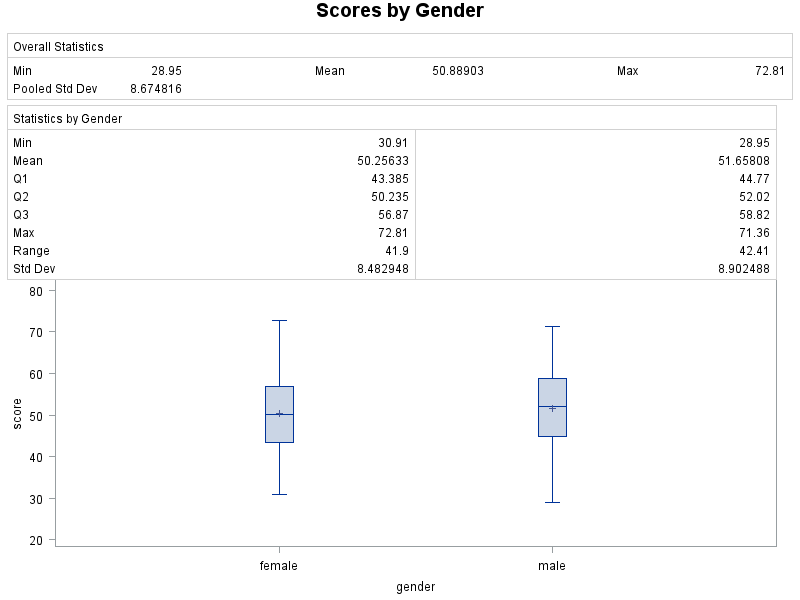
\includegraphics[width=1.14\textwidth]{images/scores_by_gender.png}
    \caption{Distribution of student scores by gender}
    \label{fig:scores_by_gender}
\end{figure}

\begin{itemize}
    \item The mean score is not significantly different based on gender, with males at 50.26 and females at 51.66
    \item The range of scores is also approximately equal, with males at 41.9 and females at 42.41
    \item Same with standard deviations, with males at 8.48 and females at 8.90
\end{itemize}
\newpage
\subsection{Distribution of "score" by Ethnicity}
\begin{figure}[h]
    \centering
    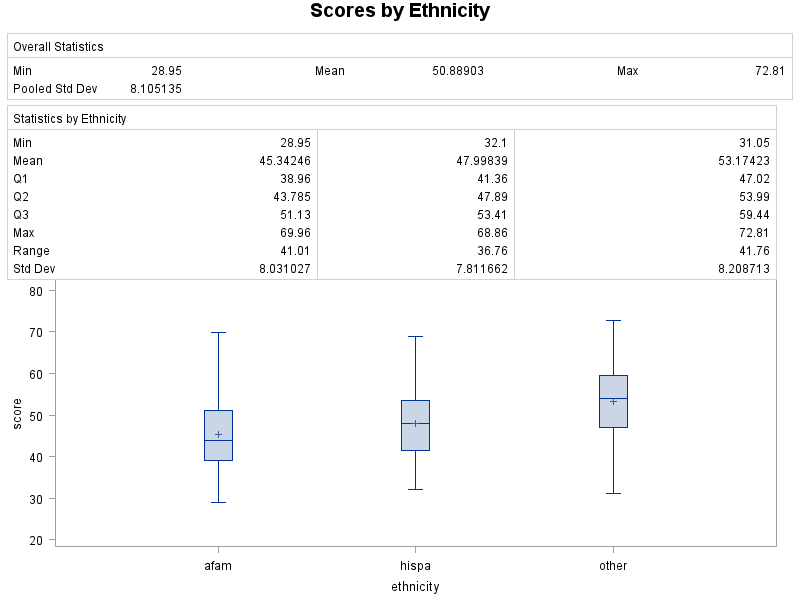
\includegraphics[width=1.14\textwidth]{images/scores_by_ethnicity.png}
    \caption{Distribution of student scores by ethnicity}
    \label{fig:scores_by_ethnicity}
\end{figure}

\begin{itemize}
    \item Average score is the highest for other ethnicities (53.17), followed by Hispanics (48) and African-Americans (45.34)
    \item The top 25\% of students of other ethnicities have a score of 59.44, followed by Hispanics (53.41) and African-Americans (51.13)
    \item The standard deviation is largest for students of other ethnicities (8.21), followed by African-Americans (8.03) and Hispanics (7.81)
\end{itemize}
\newpage
\subsection{Distribution of "score" by Father's Graduation Status}
\begin{figure}[h]
    \centering
    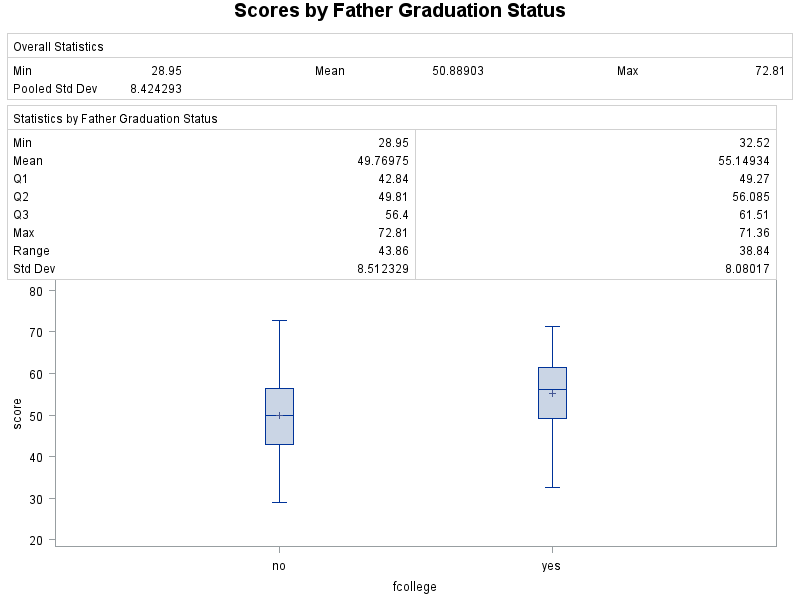
\includegraphics[width=1.14\textwidth]{images/scores_by_fcollege.png}
    \caption{Distribution of student scores by father's graduation status}
    \label{fig:scores_by_fcollege}
\end{figure}

\begin{itemize}
    \item Students have a higher average score when the father has graduated college (55.14) compared to not (49.77)
    \item Father's graduation status seems to have an effect on student performance
    \item Student scores tend to vary more for students with non-graduate parents (8.51) compared to graduates (8.08)
\end{itemize}
\newpage
\subsection{Distribution of "score" by Mother's Graduation Status}
\begin{figure}[h]
    \centering
    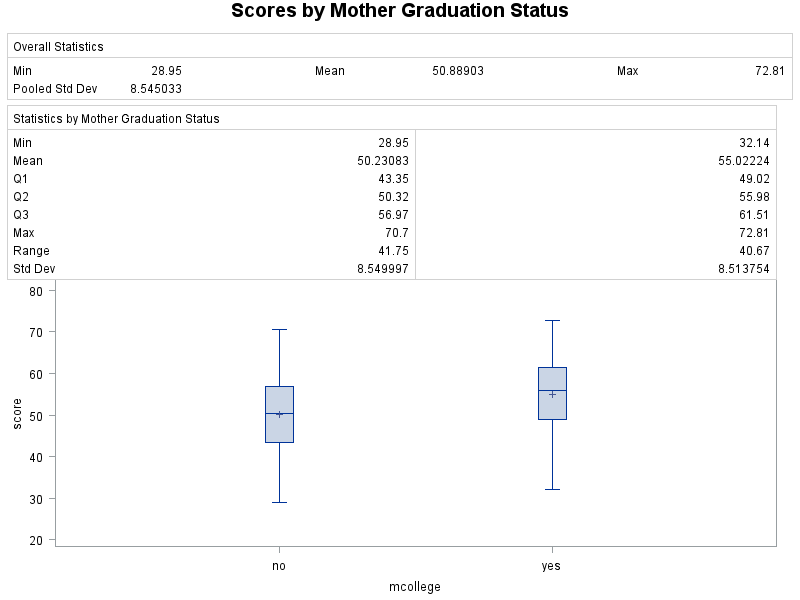
\includegraphics[width=1.14\textwidth]{images/scores_by_mcollege.png}
    \caption{Distribution of student scores by mother's graduation status}
    \label{scores_by_mcollege}
\end{figure}

\begin{itemize}
    \item A similar pattern is present when it comes to the mother's graduation status
    \item Students have a higher average score when the mother has graduated college (55.02) compared to not (50.23)
    \item Mother's graduation status seems to have an effect on student performance
\end{itemize}
\newpage
\subsection{Distribution of "score" by Home Ownership}
\begin{figure}[h]
    \centering
    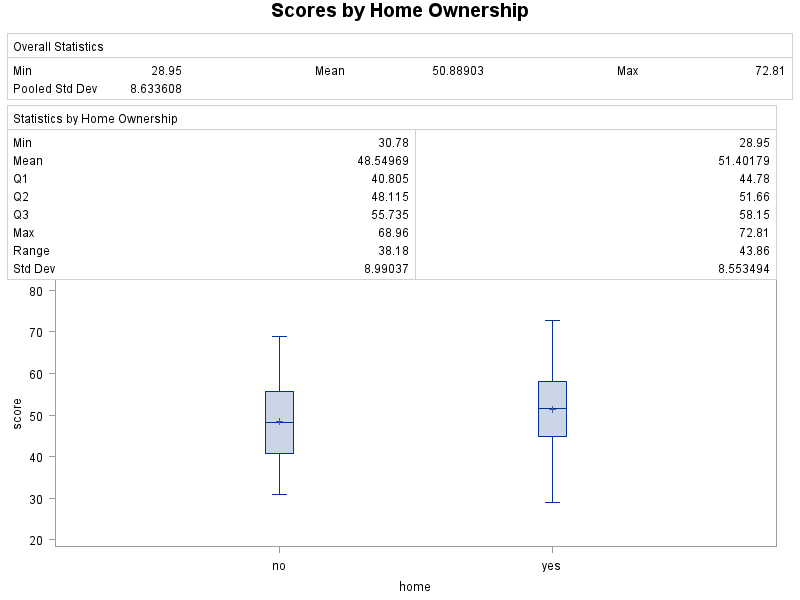
\includegraphics[width=1.14\textwidth]{images/scores_by_home.png}
    \caption{Distribution of student scores by home ownership}
    \label{scores_by_home}
\end{figure}

\begin{itemize}
    \item Student's average score is slightly higher for students that own their homes (51.40) compared to students that do not (48.55)
    \item The range of scores is larger for students that own their homes (43.86) compared to students that do not (38.18)
    \item Student scores are more dispersed for students that do not own their homes (8.99) compared to students that do (8.55)
\end{itemize}
\newpage
\subsection{Distribution of "score" by School Location}
\begin{figure}[h]
    \centering
    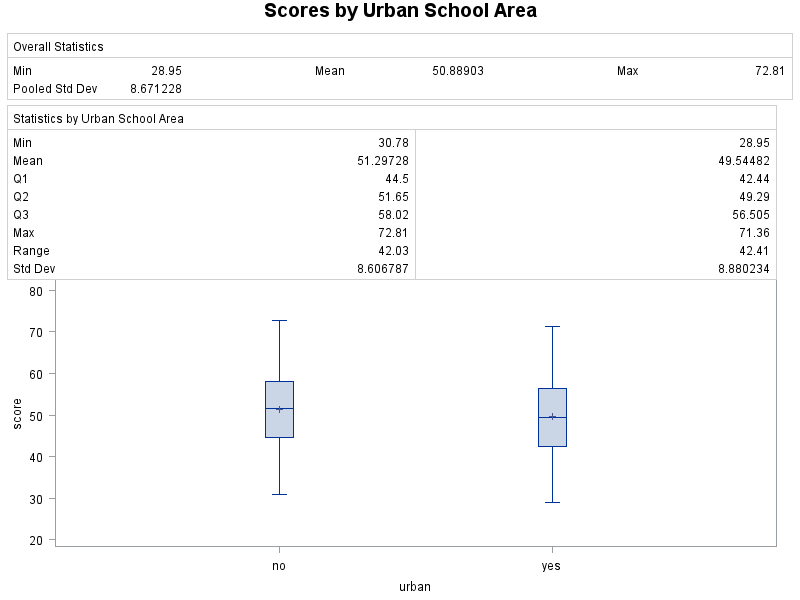
\includegraphics[width=1.14\textwidth]{images/scores_by_urban.png}
    \caption{Distribution of student scores based on whether the school is classified as urban}
    \label{scores_by_urban}
\end{figure}

\begin{itemize}
    \item Students that attend non-urban schools tend to have slightly higher scores on average (51.30) compared to urban (49.54)
    \item Range of scores is similar for both non-urban (42.03) and urban (42.41) school students
    \item Standard deviations are also similar for non-urban (8.61) and urban (8.88) school students
\end{itemize}
\newpage
\subsection{Distribution of "score" by Income Category}
\begin{figure}[h]
    \centering
    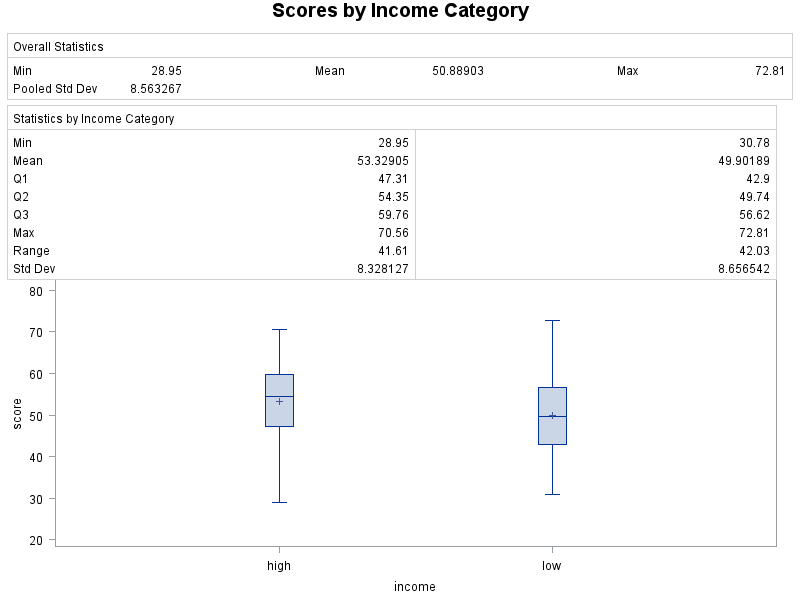
\includegraphics[width=1.14\textwidth]{images/scores_by_income_cat.png}
    \caption{Distribution of student scores based on income category}
    \label{scores_by_urban}
\end{figure}

\begin{itemize}
    \item Students that belong in the high-income category tend to score slightly higher (53.33) on average than students in the low-income category (49.90)
    \item Student scores are less dispersed for high-income students (8.33) compared to low-income (8.66)
    
\end{itemize}

\newpage

\section{Building the Linear Regression Model}
In this section, we will be creating two Linear Regression models using the adjusted R-Squared method. One will contain the previously discussed features in the dataset and the other will include interaction terms created from our features.


\subsection{Model 1: Adj. R-Squared Method}
The adjusted R-squared selection method is a technique used to assess and compare the performance of regression models. It is an extension of the traditional R-squared metric that takes into account the number of predictors in a model and adjusts for the degrees of freedom.
\begin{figure}[h]
    \centering
    \begin{minipage}[t]{0.4\textwidth}
        \vspace{10pt}
        \centering
        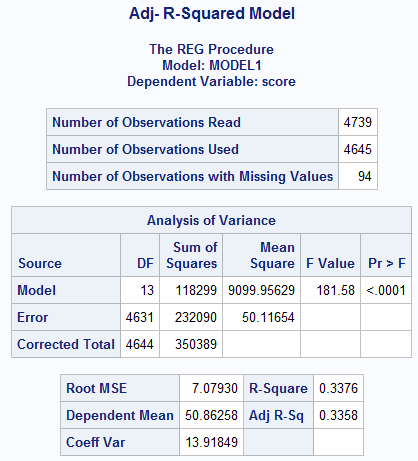
\includegraphics[width=\textwidth]{images/model1_a.png}
        % \caption{Distribution of variable "unemp"}
        \label{fig:unemp_dist}
    \end{minipage}\hfill
    \begin{minipage}[t]{0.55\textwidth}
        \vspace{0pt}
        \centering
        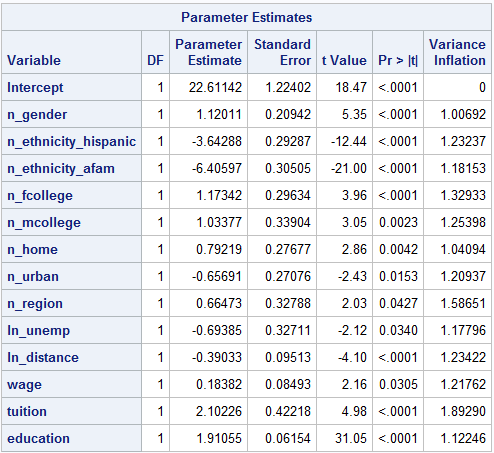
\includegraphics[width=\textwidth]{images/model1_b.png}
        
        \label{fig:unemp_measures}
    \end{minipage}
    \caption{Linear Regression model with highest adj. $R^{2}$ value}
    \label{fig:unemp_fig}
\end{figure}

 \large\noindent $H_{0}: \beta_1 = \beta_2 = ... = \beta_k = 0$\\
 $H_a:$ At least one coefficient $\beta_j \ne 0$ 
  \normalsize
\begin{itemize}
    \item This model has a total of 13 features (not including score).
    \item All of our features are statistically significant (p-value \textless .05)
    \item Our F-Statistic is 181.58, meaning our overall model as a whole is statistically significant in explaining the variation in the response variable (p-value \textless .0001)
    \item The model's $R^2$ value is 0.3376 and adjusted $R^2$ is 0.3358
    \item Root Mean Square Error is 7.07930
    \item The feature with the strongest predicting power is education (t-value=31.05, p-value\textless .0001)
    \item There is no presence of strong feature collinearity, as all of the VIF scores are below 10
\end{itemize}


\subsection{Model 2: Adj. R-Squared Method w/ Interaction Terms}
After adding multiple interaction terms to the model, the only added feature with a statistically significant effect was gender and education (p-value \textless .05). The addition of this interaction term made n\_region non-statistically significant, so it was removed from this model.
\begin{figure}[h]
    \centering
    \begin{minipage}[t]{0.4\textwidth}
        \vspace{10pt}
        \centering
        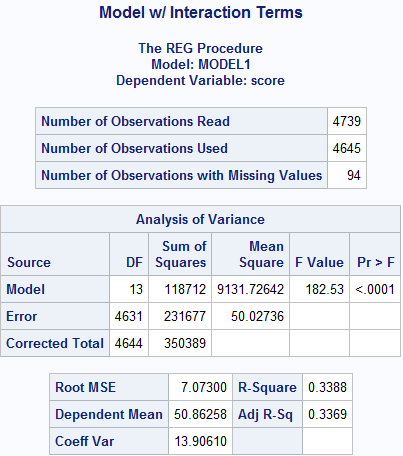
\includegraphics[width=\textwidth]{images/model2_a.png}
        % \caption{Distribution of variable "unemp"}
        \label{fig:unemp_dist}
    \end{minipage}\hfill
    \begin{minipage}[t]{0.55\textwidth}
        \vspace{0pt}
        \centering
        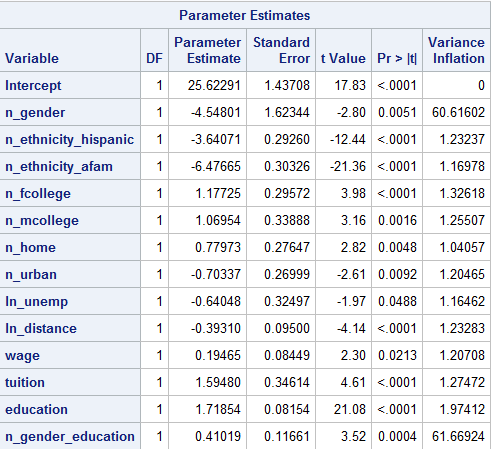
\includegraphics[width=\textwidth]{images/model2_b.png}
        
        \label{fig:unemp_measures}
    \end{minipage}
    \caption{Linear Regression model with highest adj. $R^{2}$ value and added interaction terms}
    \label{fig:unemp_fig}
\end{figure}

 \large\noindent $H_{0}: \beta_1 = \beta_2 = ... = \beta_k = 0$\\
 $H_a:$ At least one coefficient $\beta_j \ne 0$ 
  \normalsize
\begin{itemize}
    \item This model has a total of 13 features (not including score)
    \item All of our features are statistically significant (p-value \textless .05)
    \item Our F-Statistic is 182.53 with a p-value \textless .0001, meaning our overall model as a whole is statistically significant in explaining the variation in the response variable (greater than previous model)
    \item The model's $R^2$ value is 0.3388 and adjusted $R^2$ is 0.3369 (greater than previous model)
    \item Root Mean Square Error is 7.0730 (less than previous model)
    \item The feature with the strongest predicting power is n\_ethnicity\_afam (t-value=-21.36, p-value \textless .0001)
    \item Although the interaction term has a VIF greater than 10, this is to be expected when including an interaction term in the model. In addition, it has statistical significance (p-value \textless 0.05)
\end{itemize}

\section{Final Model}
After comparing both of our models on different metrics, our second model seems to be performing slightly better, with a larger F-Statistic, greater $R^2$ and adjusted $R^2$ and lesser Root Mean Square Error. We will further explore the performance of the model by analyzing its residuals.

\subsection{Residual Analysis}
\begin{figure}[h]
    \centering
    \begin{minipage}[t]{0.5\textwidth}
        \vspace{0pt}
        \centering
        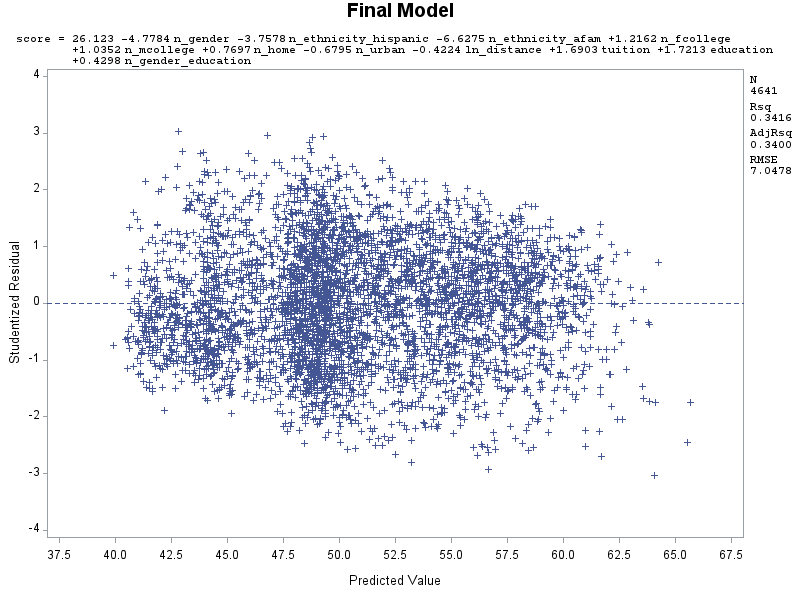
\includegraphics[width=\textwidth]{images/final_resid_pred.png}
        % \caption{Distribution of variable "unemp"}
        \label{fig:unemp_dist}
    \end{minipage}\hfill
    \begin{minipage}[t]{0.5\textwidth}
        \vspace{0pt}
        \centering
        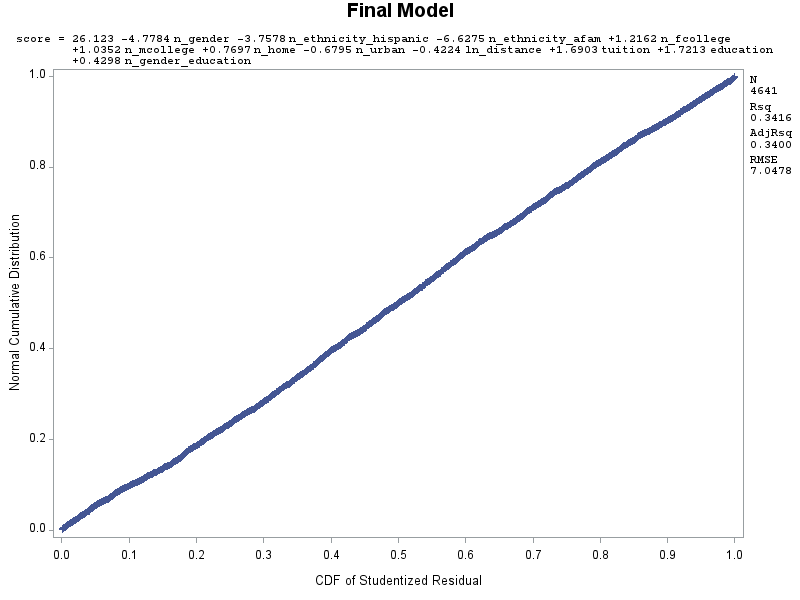
\includegraphics[width=\textwidth]{images/final_resid_cdf_ncd.png}
        
        \label{fig:unemp_measures}
    \end{minipage}
    \caption{Studentized residuals for the final model}
    \label{fig:unemp_fig}
\end{figure}

The studentized residual of the model is normally distributed when plotted against the Normal Cumulative Distribution. Also, the studentized residual for the predicted variable does not have any strong patterns present and is randomly distributed. However, some residuals are greater than 3 standard deviations away from the center. These points could be outliers that are influencing our model output. We will check for outliers and influential points in the dataset.

\newpage
\subsection{Outliers and Influential Points}

\begin{figure}[h]
    \centering
    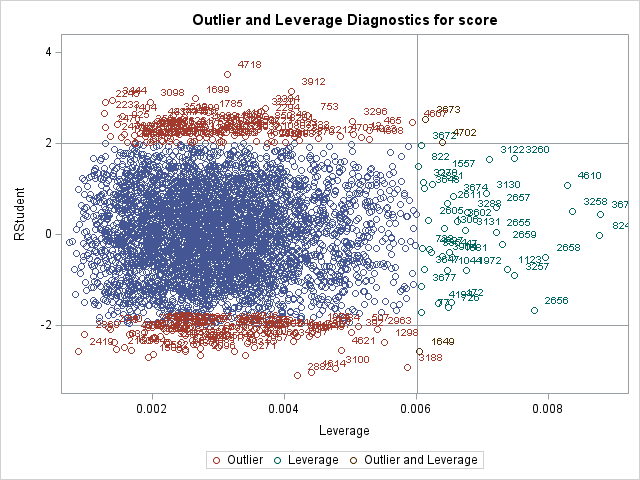
\includegraphics[width=\textwidth]{images/outlier_leverage.png}
    \caption{Outlier and leverage graph based on Student's R and Leverage}
    \label{fig:enter-label}
\end{figure}

Our dataset contains quite a few records that have a studentized residual greater or lesser than 3 standard deviations from the center. In addition, a few data points have leverage greater than 0.006 (2p/n, p=14, n=4,739). These datapoints will be removed, leaving us with a total of 4,641 observations.

\subsection{Final Model}
Upon removing all outliers and influential points from the dataset, it was observed that the variables "wage" and "ln\_unemp" exhibited no statistically significant relationship (p-value \textgreater .05). After removing these variables, we are left with 11 predictors.
\begin{figure}[h]
    \centering
    \begin{minipage}[t]{0.4\textwidth}
        \vspace{10pt}
        \centering
        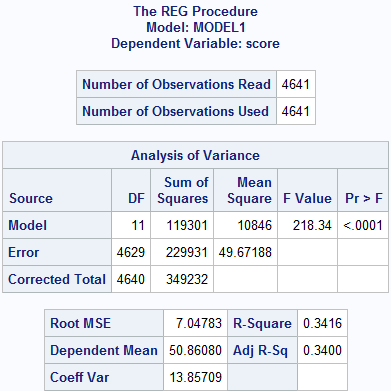
\includegraphics[width=\textwidth]{images/final_model1.png}
        % \caption{Distribution of variable "unemp"}
        \label{fig:unemp_dist}
    \end{minipage}\hfill
    \begin{minipage}[t]{0.55\textwidth}
        \vspace{0pt}
        \centering
        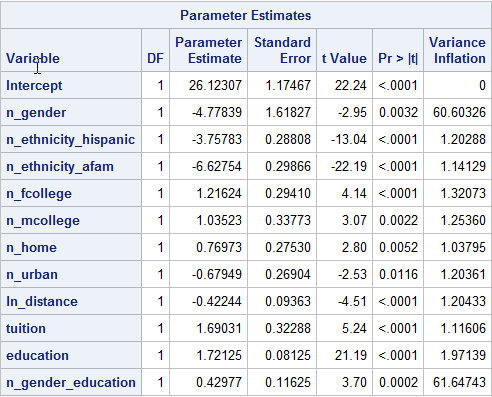
\includegraphics[width=\textwidth]{images/final_model2.png}
        
        \label{fig:unemp_measures}
    \end{minipage}
    \caption{Linear Regression model with highest adj. $R^{2}$ value and added interaction terms}
    \label{fig:unemp_fig}
\end{figure}

 \large\noindent $H_{0}: \beta_1 = \beta_2 = ... = \beta_k = 0$\\
 $H_a:$ At least one coefficient $\beta_j \ne 0$ 
  \normalsize
\begin{itemize}
    \item This model has a total of 11 features (not including score)
    \item All of our features are statistically significant (p-value \textless .05)
    \item Our F-Statistic is 218.34 with a p-value \textless .0001, much greater than any previous model
    \item The model's $R^2$ value is 0.3416 and adjusted $R^2$ is 0.34, which is also greater than the previous models
    \item Root Mean Square Error is 7.04783
    \item The feature with the strongest predicting power is n\_ethnicity\_afam (t-value=-22.19, p-value \textless .0001)
\end{itemize}

\subsection{Parameter Estimates}
\begin{itemize}
    \item n\_gender: Student score decreases by 4.77\% when the student is male
    \item n\_ethnicity\_hispanic: Student score decreases by 3.76\% when the student is Hispanic compared to other students (control group=n\_ethnicity\_other)
    \item n\_ethnicity\_afam: Student score decreases by 6.63\% when the student is African American compared to other students
    \item n\_fcollege: Student scores increases by 1.22\% when the father is a graduate
    \item n\_mcollege: Student score increases by 1.04\% when the mother is a graduate
    \item n\_home: Student score increases by 0.77\% when their family owns their home
    \item n\_urban: Student score decreases by 0.68\% when the school is in an urban area
    \item ln\_distance: Student score decreases by (exp(-0.42)-1)*100 = 34\% for each additional 10 miles in distance (1 unit=10 miles)
    \item tuition: Student score increases by 1.69\% for every \$1000 in tuition
    \item education: Student score increases by 0.43\% for each additional year of education when the gender is female (n\_gender=0)
    \item n\_gender\_education: Student score increases by (1.72+0.43 = ) 2.5\% for each additional year of education when the gender is male (n\_gender=1)
\end{itemize}

\section{Training and Testing}
Our dataset will be split into 80\% training and 20\% testing randomly. 

\subsection{Training Results}
\begin{figure}[h]
    \centering
    \begin{minipage}[t]{0.4\textwidth}
        \vspace{10pt}
        \centering
        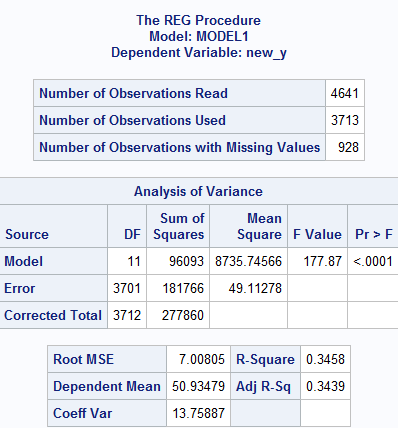
\includegraphics[width=\textwidth]{images/training_model1.png}
        % \caption{Distribution of variable "unemp"}
        \label{fig:unemp_dist}
    \end{minipage}\hfill
    \begin{minipage}[t]{0.55\textwidth}
        \vspace{0pt}
        \centering
        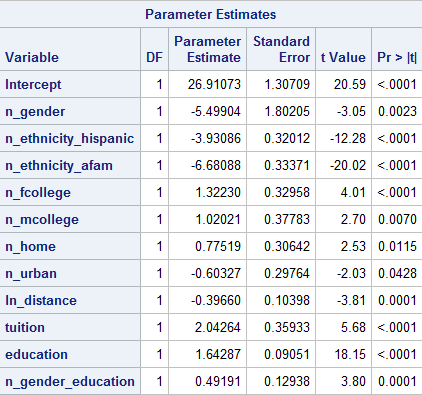
\includegraphics[width=\textwidth]{images/training_model2.png}
        
        \label{fig:unemp_measures}
    \end{minipage}
    \caption{Linear Regression model model results on training set}
    \label{fig:unemp_fig}
\end{figure}
\begin{itemize}
    \item Our F-Statistic for the training data is 177.87 with a p-value \textless .0001
    \item The model's $R^2$ value is 0.3458 and adjusted $R^2$ is 0.3439
    \item Root Mean Squared Error is 7.00805
\end{itemize}

\subsection{Testing Results}
\begin{figure}[h]
    \centering
    \begin{minipage}[t]{0.4\textwidth}
        \vspace{40pt}
        \centering
        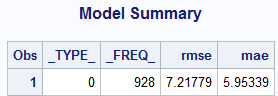
\includegraphics[width=\textwidth]{images/testing_model1.png}
        % \caption{Distribution of variable "unemp"}
        \label{fig:unemp_dist}
    \end{minipage}\hfill
    \begin{minipage}[t]{0.55\textwidth}
        \vspace{0pt}
        \centering
        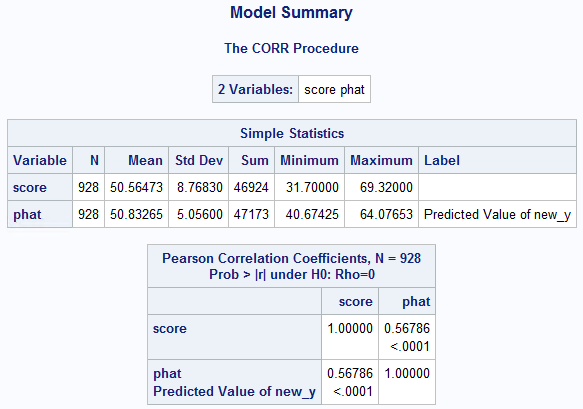
\includegraphics[width=\textwidth]{images/testing_model2.png}
        
        \label{fig:unemp_measures}
    \end{minipage}
    \caption{Linear Regression model model results on testing set}
    \label{fig:unemp_fig}
\end{figure}

\newpage
\begin{itemize}
    \item Root Mean Squared Error= 7.21779
    \item $R^2$= $\hat{p}^2$= 0.32246498
    \item CV $R^2$= 0.3458 - 0.32246498= 0.02333502
\end{itemize}
Our model is performing equally well on the testing set as on the training set. RMSE and $R^2$ do not wildly differ from each other in both cases, meaning the model is not overfitting the training data.

\subsection{Testing Model on New Records}
After training and testing the model on the previous dataset, we will create some new records and see how the model performs on previously unseen data.
\begin{figure}[h]
    \centering
    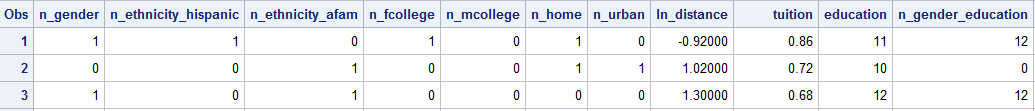
\includegraphics[width=\textwidth]{tables/new_records.png}
    \caption{New records manually created to test the model}
    \label{fig:enter-label}
\end{figure}
\begin{figure}[h]
    \centering
    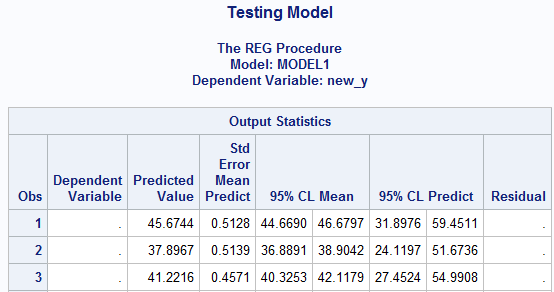
\includegraphics[width=\textwidth]{images/test_new.png}
    \caption{Testing model performance on new unseen records}
    \label{fig:enter-label}
\end{figure}
\newpage
\begin{itemize}
    \item Obs. 1: Predicted= 45.6744, CI= [31.8976, 59.4511]
    \item Obs. 2: Predicted= 37.8967, CI= [24.1197, 51.6736]
    \item Obs. 3: Predicted= 41.2216, CI= [27.4524, 54.9908]
\end{itemize}
\end{document}











